\documentclass[11pt,a4paper]{article}

\usepackage[a4paper,margin=25mm]{geometry}
\usepackage[T1]{fontenc}
\usepackage[utf8]{inputenc}
\usepackage{lmodern}
\usepackage{microtype}
\usepackage{graphicx}
\usepackage{subcaption}
\usepackage{booktabs}
\usepackage{array}
\usepackage{longtable}
\usepackage{enumitem}
\usepackage{xcolor}
\usepackage{hyperref}
\usepackage{caption}
\usepackage{fancyhdr}
\usepackage{titlesec}

\graphicspath{{../../}}

\definecolor{octaneorange}{HTML}{D86B1F}
\definecolor{octaneblue}{HTML}{1E5B8E}
\definecolor{softgray}{HTML}{F3F4F6}
\definecolor{darkgray}{HTML}{333333}

\hypersetup{
  colorlinks=true,
  linkcolor=octaneblue,
  urlcolor=octaneblue,
  citecolor=octaneblue,
  pdftitle={OctaneX MCP: Conceptual Design and Operating Principles},
  pdfauthor={Craig Stone / Hermes Agent},
  pdfsubject={Local MCP bridge for agentic Octane X visualization}
}

\pagestyle{fancy}
\fancyhf{}
\lhead{OctaneX MCP Whitepaper}
\rhead{\thepage}
\setlength{\headheight}{14pt}
\emergencystretch=2em

\titleformat{\section}{\Large\bfseries\color{octaneblue}}{\thesection}{0.75em}{}
\titleformat{\subsection}{\large\bfseries\color{darkgray}}{\thesubsection}{0.75em}{}

\newcommand{\project}{OctaneX MCP}
\newcommand{\mcp}{MCP}
\newcommand{\figpath}[1]{../../#1}

\title{\vspace{-1em}\textbf{OctaneX MCP}\\[0.35em]
\large Conceptual Design, Operating Principles, and Application Roadmap}
\author{Craig Stone \and Hermes Agent}
\date{Draft whitepaper --- July 2026}

\begin{document}
\maketitle

\begin{abstract}
\project{} is a local-first Model Context Protocol server that lets an agent use Octane X as a shared visual canvas. Instead of treating image generation as a single text-to-image request, it constructs explicit scene geometry, material intent, camera placement, lighting, render commands, and pixel-level verification loops. The current implementation routes Hermes tool calls through a Python MCP server, an allowlisted JSON command queue, and an Octane Lua bridge that executes bounded scene operations inside Octane X. This whitepaper describes the project's conceptual design, operating principles, recipe corpus, comparison with other image/model generation toolsets, planned development path, and application opportunities. It uses examples from the recent recipe corpus, including product-studio objects, Earth and planetary scenes, architecture/data/math visuals, and feedback-loop diagrams.
\end{abstract}

\tableofcontents
\newpage

\section{Executive summary}

\project{} is best understood as a \emph{visual workbench for agents}, not a conventional image generator. Its goal is to make rendered scenes inspectable, reproducible, and editable by local AI agents. The project currently provides:

\begin{itemize}[leftmargin=*]
  \item a Python MCP server exposing Octane-oriented tools to Hermes;
  \item a typed, allowlisted command schema for mesh import, material creation, material assignment, camera placement, lighting, rendering, preview saving, recipe loading, and review;
  \item a macOS Octane X bridge implemented as Lua scripts that drain JSON command files from a sandbox-compatible workspace;
  \item a growing recipe corpus of 30 checked-in scene directories, 25 of which currently declare native Octane verification and 29 of which carry preview imagery;
  \item a benchmark suite and pixel-level acceptance framework that evaluates renders through decoded image statistics rather than model opinion;
  \item a documentation and recipe-book layer that captures operational lessons for smaller/local models.
\end{itemize}

The central design choice is to keep scene construction explicit. Text-to-image systems such as Stable Diffusion, FLUX, Midjourney-style services, and ComfyUI graphs can produce compelling images quickly, but they usually collapse geometry, material, camera, and provenance into latent state. \project{} instead preserves a concrete scene artifact: OBJ/MTL geometry, command metadata, material groups, camera bounds, preview output, and verification results. That makes it better suited to scientific visualization, geospatial explanation, reproducible diagrams, product-style iteration, and agent learning loops where the system must know \emph{what changed} between renders.

\section{Motivation}

Visual explanation is a recurring bottleneck in exploratory research and software development. The user often needs to inspect geometry, compare hypotheses, explain a pipeline, or communicate a concept visually. Existing generative-image tools are strong at style and composition but weak at deterministic editability. Traditional rendering tools are powerful but require manual operation and do not naturally expose an agent-readable contract.

\project{} addresses the gap by connecting a local agent to a professional renderer through a restricted command protocol. The result is a shared visual medium with three properties:

\begin{enumerate}[leftmargin=*]
  \item \textbf{Reproducibility.} A scene is built from files, JSON commands, camera parameters, and recipe metadata, not from an opaque latent prompt alone.
  \item \textbf{Inspectability.} A rendered preview is checked by pixel metrics and, when useful, by a local vision model for human-facing description. Pixel metrics remain the pass/fail gate.
  \item \textbf{Iterability.} Failures become bounded edits: adjust the camera, change material opacity, regenerate geometry, or requeue a recipe. Successful patterns become reusable recipes.
\end{enumerate}

This framing is especially useful for Craig Stone's work across geospatial analysis, math/geometry visualisation, scientific illustration, agentic render workflows, and local-first AI tooling. A rendered scene becomes an artifact that can be versioned, tested, and improved.

\section{Conceptual architecture}

At the highest level, \project{} separates three concerns: agent intent, scene/command generation, and renderer execution. Hermes supplies the intent and tool call. The Python MCP server validates that intent and emits a safe command sequence. Octane X executes the sequence only through a Lua bridge inside the renderer.

\begin{figure}[htbp]
\centering
\fbox{\begin{minipage}{0.92\linewidth}
\centering
\vspace{0.8em}
\texttt{Hermes tool call} $\rightarrow$ \texttt{Python MCP server} $\rightarrow$ \texttt{JSON command queue}\\[0.4em]
$\rightarrow$ \texttt{Octane Lua bridge} $\rightarrow$ \texttt{Octane X scene/render target} $\rightarrow$ \texttt{PNG preview + review}
\vspace{0.8em}
\end{minipage}}
\caption{Current operating pipeline. The MCP server does not run arbitrary Lua. It writes an allowlisted command DSL into a workspace queue; Octane X processes that queue through generated Lua bridge scripts.}
\label{fig:pipeline}
\end{figure}

\subsection{Core components}

\begin{description}[leftmargin=!,labelwidth=36mm]
  \item[Python MCP server] Provides tool surfaces such as status checks, schema inspection, geometry import, material creation, recipe indexing/loading/queueing, scene-plan construction, animation command generation, and preview review.
  \item[Typed command schema] Defines supported operations and payload validation. This is the main safety boundary: commands are explicit and bounded rather than arbitrary code.
  \item[Workspace queue] Stores ordered JSON command files under the Octane X sandbox-compatible workspace. Lifecycle directories include \texttt{queue/}, \texttt{processing/}, \texttt{processed/}, \texttt{failed/}, \texttt{results/}, \texttt{assets/}, and \texttt{renders/}.
  \item[Lua bridge] Runs inside Octane X from the Script menu. The one-shot bridge drains the queue and exits; the persistent bridge is available for manual/timer-style operation, but the one-shot path is the preferred batch mechanism.
  \item[Recipe corpus] Stores reusable scene directories with geometry, material files, scene metadata, preview imagery, and operational notes.
  \item[Review layer] Decodes PNG output to detect blank frames, clipping, low contrast, foreground size, and other failure modes. Vision models may assist interpretation, but decoded pixels remain the truth source.
\end{description}

\subsection{Operating principle: explicit scene state}

The project deliberately makes geometry and scene intent first-class. A recipe is not merely a prompt; it is a directory with files such as:

\begin{itemize}[leftmargin=*]
  \item \texttt{scene.obj}: renderable geometry;
  \item \texttt{scene.mtl}: material-group hints;
  \item \texttt{scene.json}: command metadata, camera, lighting, domains, verification flags, and purpose;
  \item \texttt{octane-preview.png}: native Octane preview when available;
  \item \texttt{README.md}: prompt, usage notes, variations, and pitfalls.
\end{itemize}

This means later agents can inspect the actual assets, requeue them, compare outputs, and update the recipe with evidence rather than guessing from prose.

\section{Operating principles}

\subsection{Local-first control}

The project is designed around local execution. Hermes runs locally, Octane X runs locally, and rendered previews are written into local workspace folders. This aligns with privacy, reproducibility, and the ability to use local models for visual critique and documentation work.

\subsection{Allowlisted execution}

The bridge intentionally avoids arbitrary Lua execution. The Python side emits a controlled command language with operations such as import geometry, create material, assign material, set camera, set lighting, save preview, and validate queue. The Lua side dispatches only recognized operations. Invalid commands are moved to failure paths with metadata.

\subsection{Pixel truth before model opinion}

A central lesson of the project is that vision models can hallucinate correctness. The benchmark suite and recipe-verification protocol therefore treat decoded image statistics as the pass/fail layer. A preview must not be blank, clipped, near-black, or otherwise structurally wrong merely because a captioning model describes it optimistically.

\subsection{One-shot queue draining}

The robust current path is to queue a complete scene pipeline and run the one-shot Lua bridge once. One click drains the whole queue. This reduces viewport staleness and avoids partial-scene states where geometry imports but materials, cameras, or preview saves do not arrive in the intended order.

\subsection{Recipe learning loop}

Every non-trivial success, failure, or pitfall can be recorded in the recipe book. This turns individual render sessions into project memory. The aim is not just to make images, but to teach later agents exactly how a scene was built, verified, and corrected.

\section{Current implementation status}

The current repository state, as captured in the project status documents, is a working visual workbench with a live bridge, broad unit coverage, 30 recipe directories, a growing corpus of native previews, and an active roadmap for bridge hardening and backend abstraction. The principal live constraints are not conceptual viability, but operational integration details: macOS sandbox paths, Accessibility/TCC permissions for AppleScript launch, Octane's Script-menu workflow, queue hygiene, and drift between rapidly evolving recipes and documentation.

\begin{table}[htbp]
\centering
\caption{Current capability snapshot distilled from project docs and recipe metadata.}
\begin{tabular}{p{0.30\linewidth}p{0.58\linewidth}}
\toprule
\textbf{Area} & \textbf{State} \\
\midrule
MCP server & Python stdio server with tool catalogue, schema, recipe registry, preview review, scene-plan helpers, and animation command generation. \\
Command transport & Ordered JSON queue processed by Octane-side Lua scripts. \\
Renderer & Octane X, currently controlled via macOS Script-menu bridge rather than a formal CLI/plugin API. \\
Recipe corpus & 30 recipe directories; 25 currently declare native Octane verification; 29 carry preview imagery. \\
Verification & Unit tests, benchmark suite, recipe validation, pixel QA, and local visual inspection where appropriate. \\
Open bridge work & Single-source Lua handler generation, capability-backed material/light registry, richer backend abstraction. \\
Open application work & 3DXM parametric/Weierstrass meshing, geospatial live path, short orbit clips, Agentic Canvas status/operator surface. \\
\bottomrule
\end{tabular}
\end{table}

\section{Recipe corpus as evidence}

The recipe corpus is the practical proof of the design. It demonstrates that the bridge can support more than a test cube: product geometry, scientific scenes, data diagrams, architecture flows, planetary scenes, and agent-feedback diagrams can all be represented as explicit geometry and re-rendered.

\subsection{Recent product and object recipes}

\begin{figure}[htbp]
\centering
\begin{subfigure}{0.32\linewidth}
  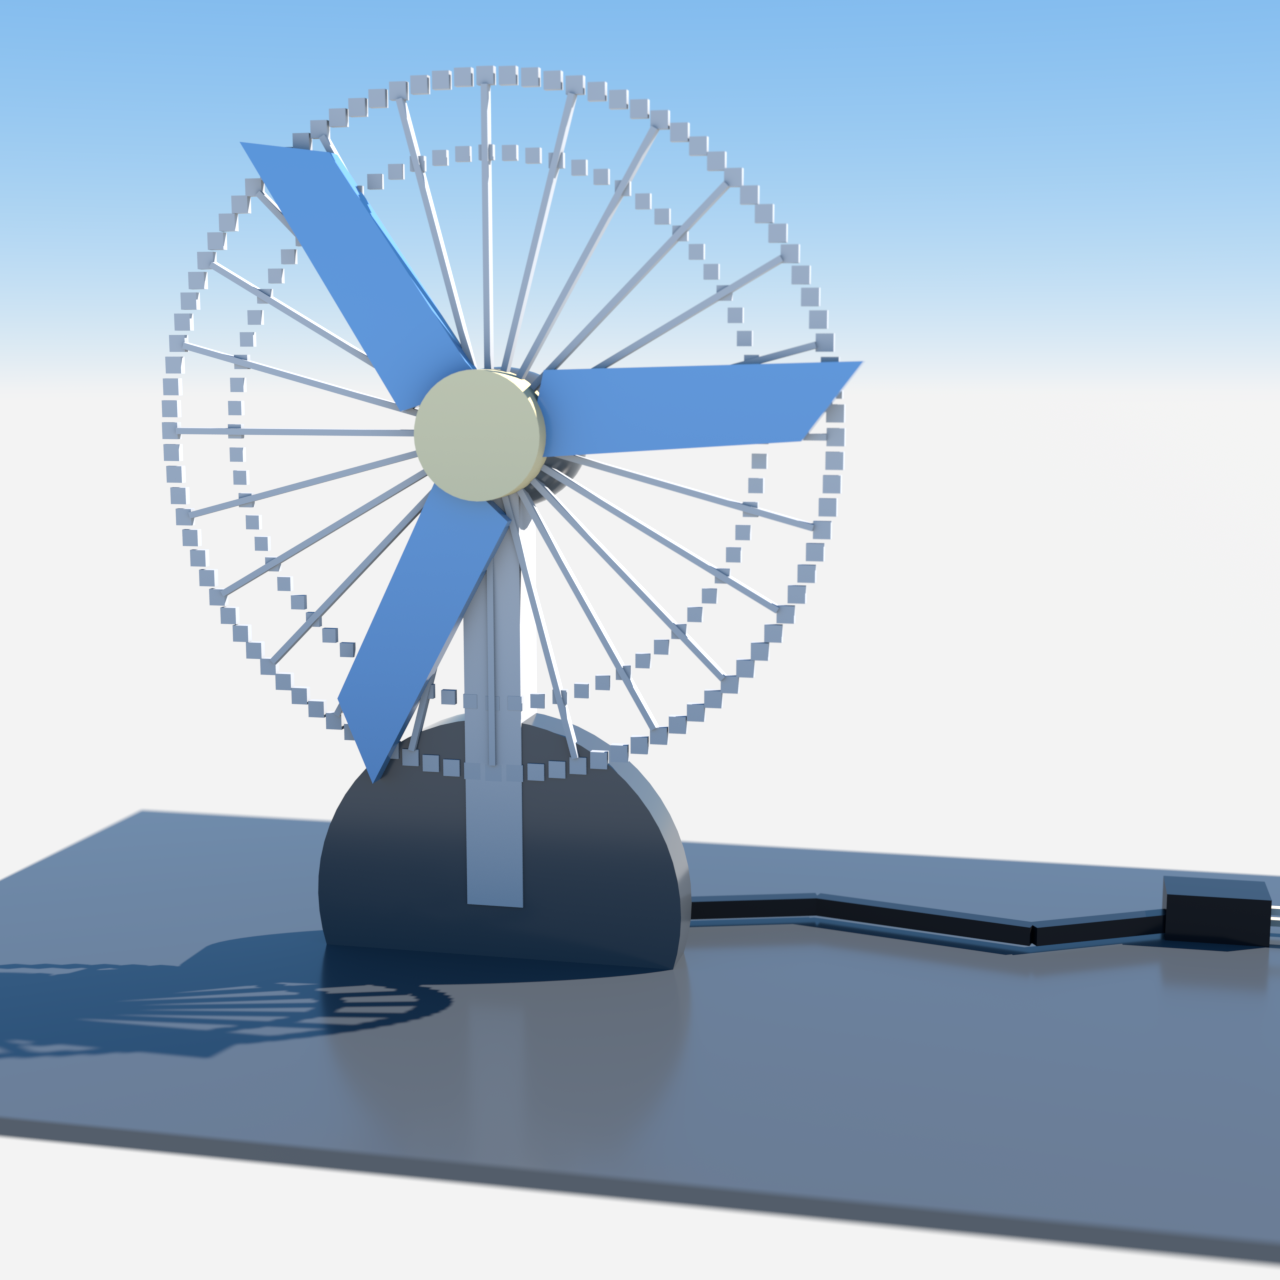
\includegraphics[width=\linewidth]{examples/recipes/desk-fan/octane-preview.png}
  \caption{Desk fan with cage, blades, cord, plug, and brass prongs.}
\end{subfigure}\hfill
\begin{subfigure}{0.32\linewidth}
  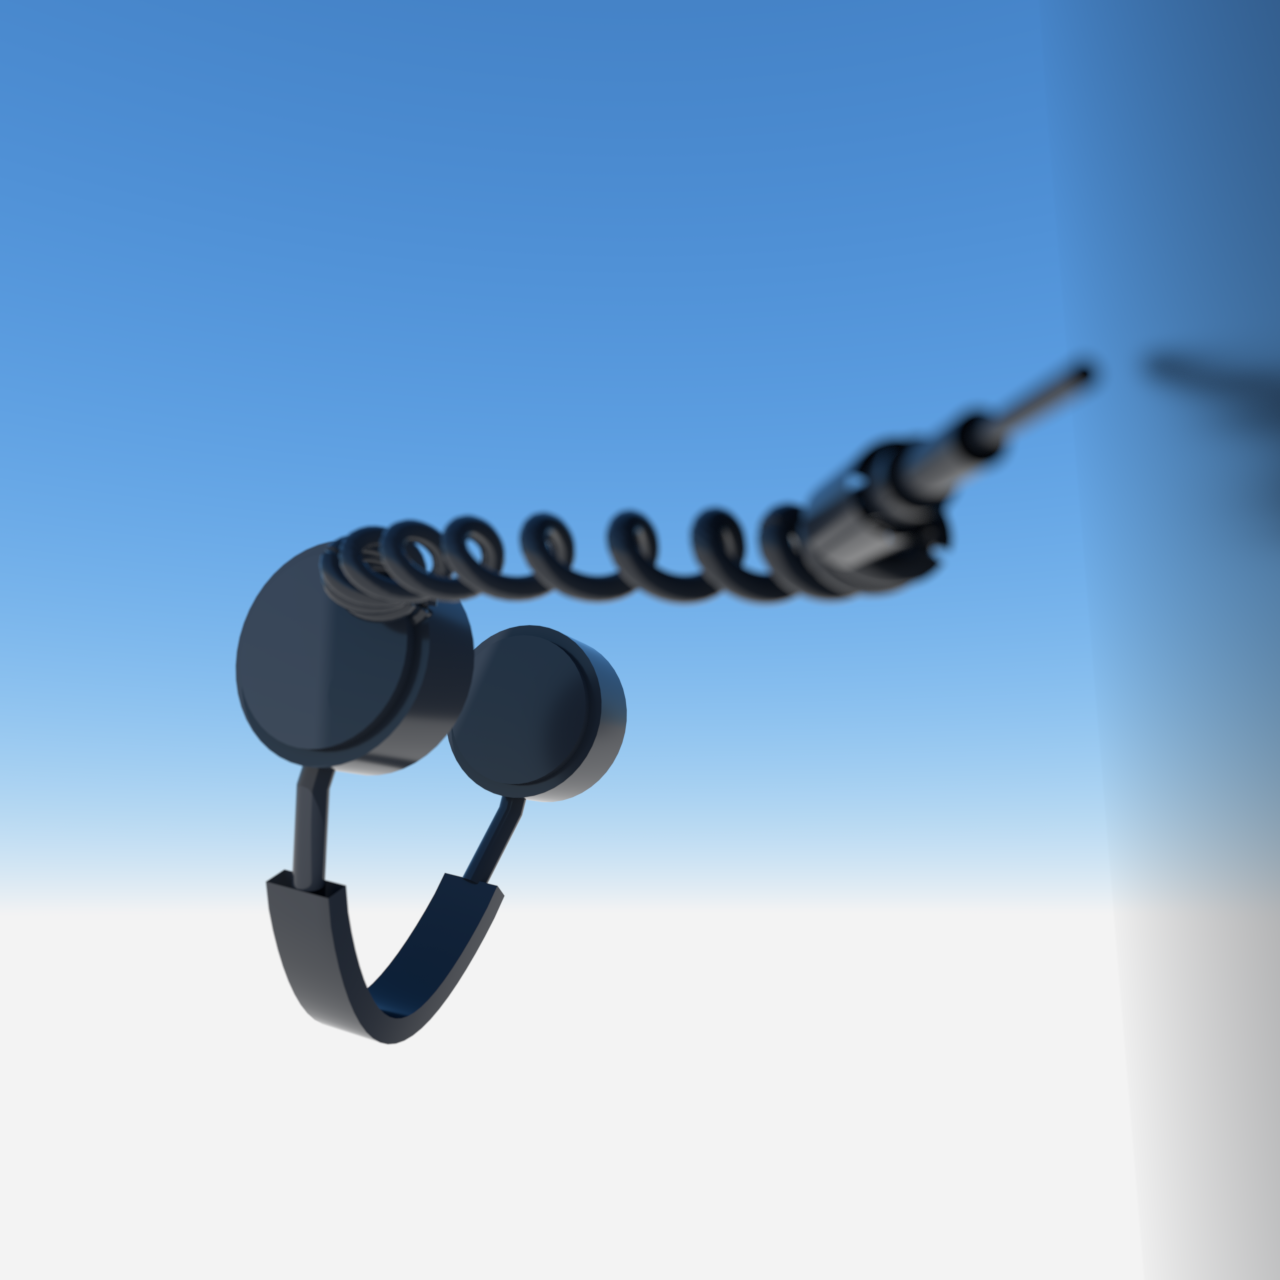
\includegraphics[width=\linewidth]{examples/recipes/headphones-studio/octane-preview.png}
  \caption{Over-ear headphones with opposing cylindrical cups and spiral cord.}
\end{subfigure}\hfill
\begin{subfigure}{0.32\linewidth}
  
\includegraphics[width=\linewidth]{examples/recipes/photoreal-vase-studio/octane-preview.png}
  \caption{Multi-vase studio target with glass, ceramic, terracotta, marble, and metal cues.}
\end{subfigure}
\caption{Product-style recipes show the value of explicit geometry: user feedback can target concrete elements such as cup orientation, cable topology, cap faces, cage wires, material groups, or camera focus.}
\label{fig:product-recipes}
\end{figure}

These recipes illustrate why \project{} differs from prompt-only image generation. In the desk-fan and headphones examples, iteration was about specific 3D structure: closed cylinders, rotated earcups, tubular cords, guard wires, plug prongs, and grounding shadows. Those details are easier to correct when the scene is generated as geometry rather than inferred in a latent image.

\subsection{Scientific and planetary recipes}

\begin{figure}[htbp]
\centering
\begin{subfigure}{0.32\linewidth}
  
\includegraphics[width=\linewidth]{examples/recipes/earth-hemisphere/octane-preview.png}
  \caption{Cutaway Earth point cloud with glowing core, mantle/crust layers, and atmosphere.}
\end{subfigure}\hfill
\begin{subfigure}{0.32\linewidth}
  
\includegraphics[width=\linewidth]{examples/recipes/photoreal-earth-space/octane-preview.png}
  \caption{Orbital Earth scene with clouds, atmosphere rim, and space lighting.}
\end{subfigure}\hfill
\begin{subfigure}{0.32\linewidth}
  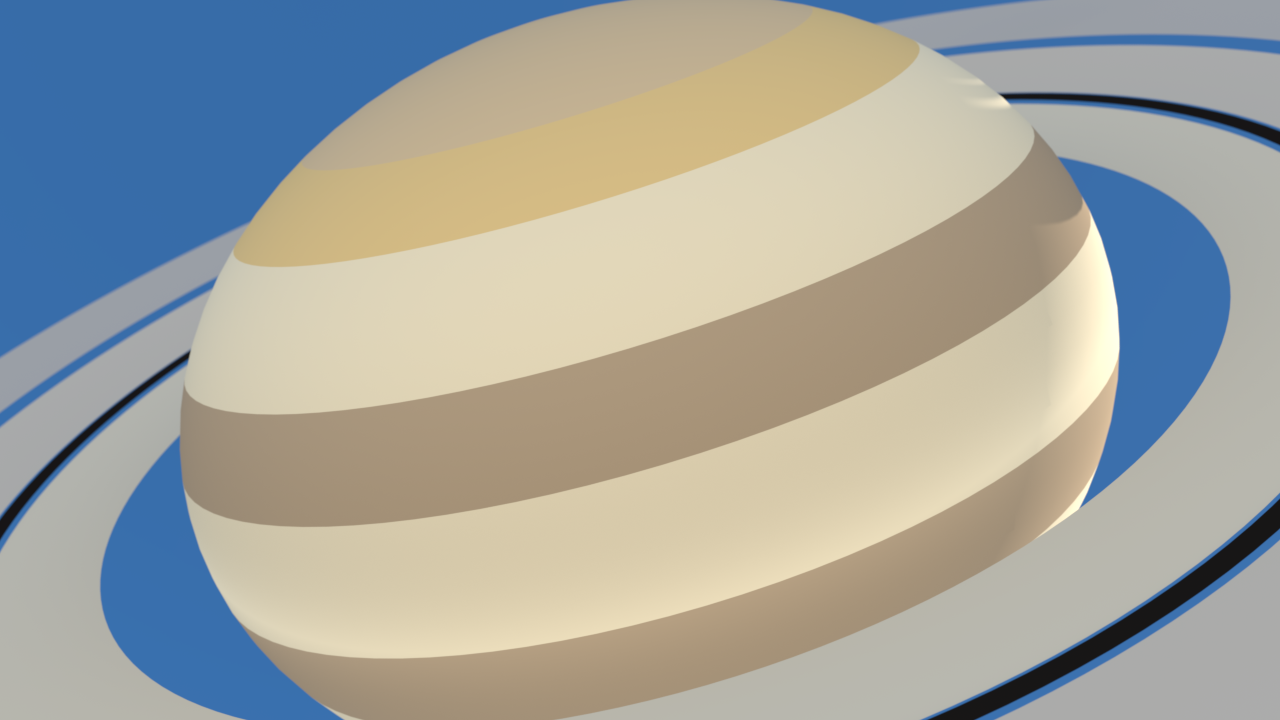
\includegraphics[width=\linewidth]{examples/recipes/saturn-moons-space/octane-preview.png}
  \caption{Saturn scene with oblate planet, rings, moons, and cinematic lighting.}
\end{subfigure}
\caption{Planetary and geoscience recipes demonstrate the project's research-visualisation direction: structured geometry plus material semantics, not only visual style.}
\label{fig:planet-recipes}
\end{figure}

The Earth cutaway is a particularly important stress case. It uses a dense point-cloud representation with grouped layers, opacity, emission, atmosphere shells, and off-axis camera choices. The recipe-book notes show how failures are turned into concrete next actions: change the camera angle when the cutaway reads as a flat disc, sweep stranded \texttt{processing/} commands back into the job, and verify material-group counts before promotion.

\subsection{Data, graph, and architecture recipes}

\begin{figure}[htbp]
\centering
\begin{subfigure}{0.32\linewidth}
  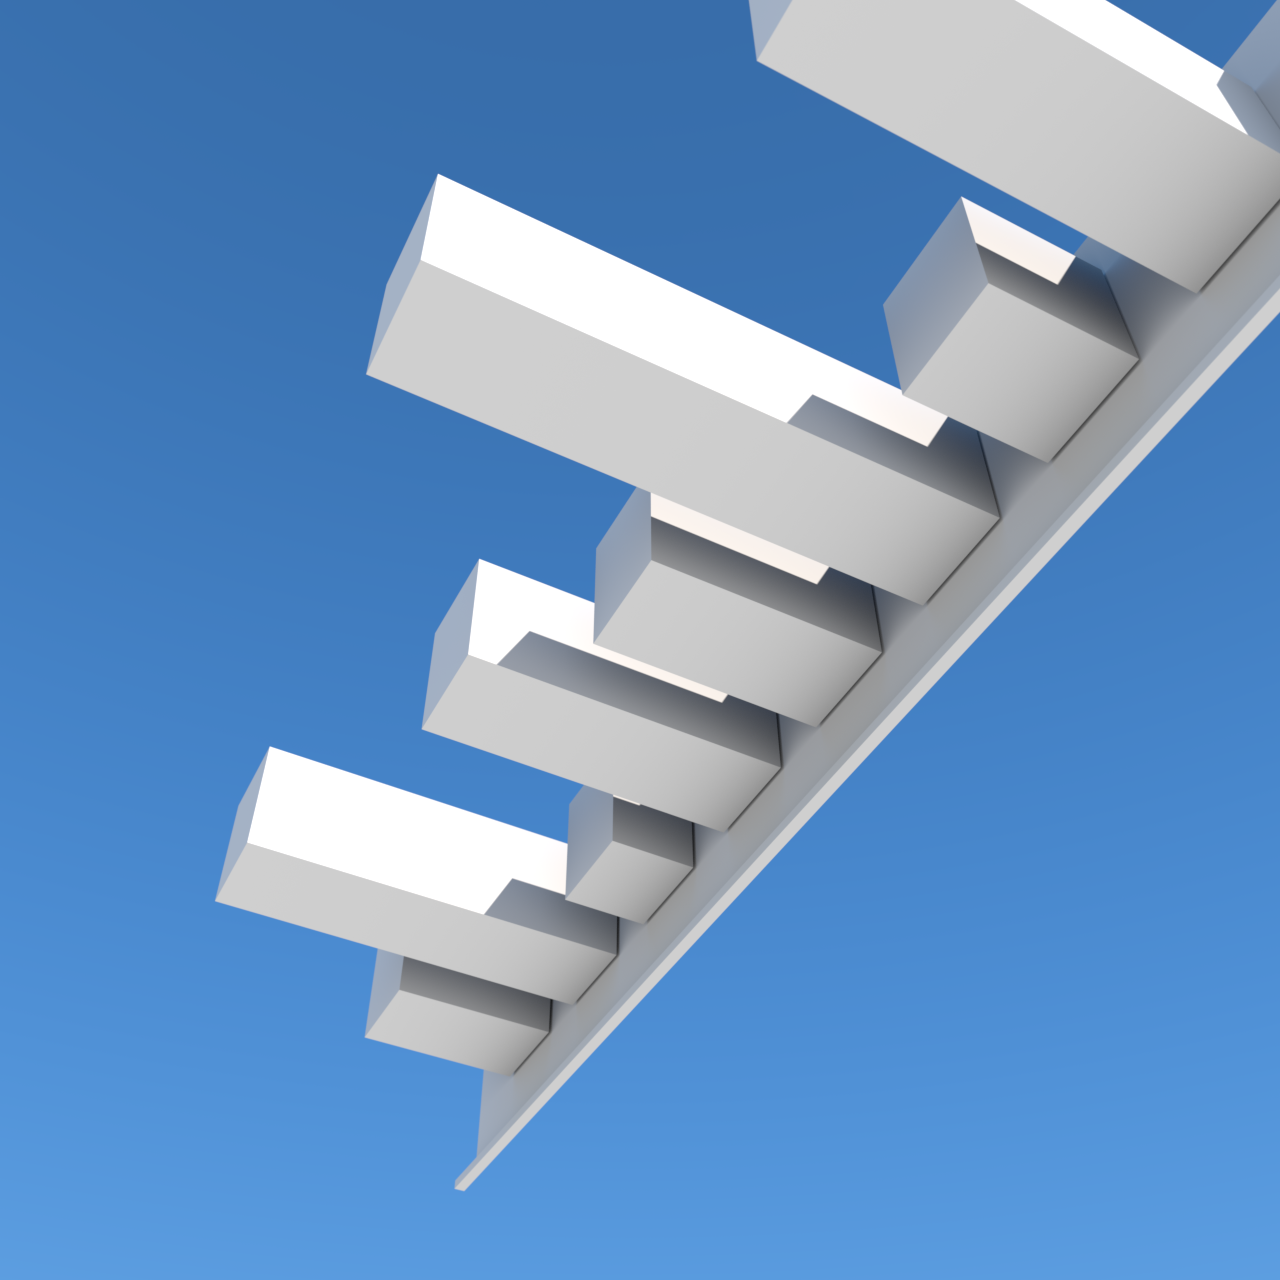
\includegraphics[width=\linewidth]{examples/recipes/data-bars/octane-preview.png}
  \caption{3D KPI bar chart.}
\end{subfigure}\hfill
\begin{subfigure}{0.32\linewidth}
  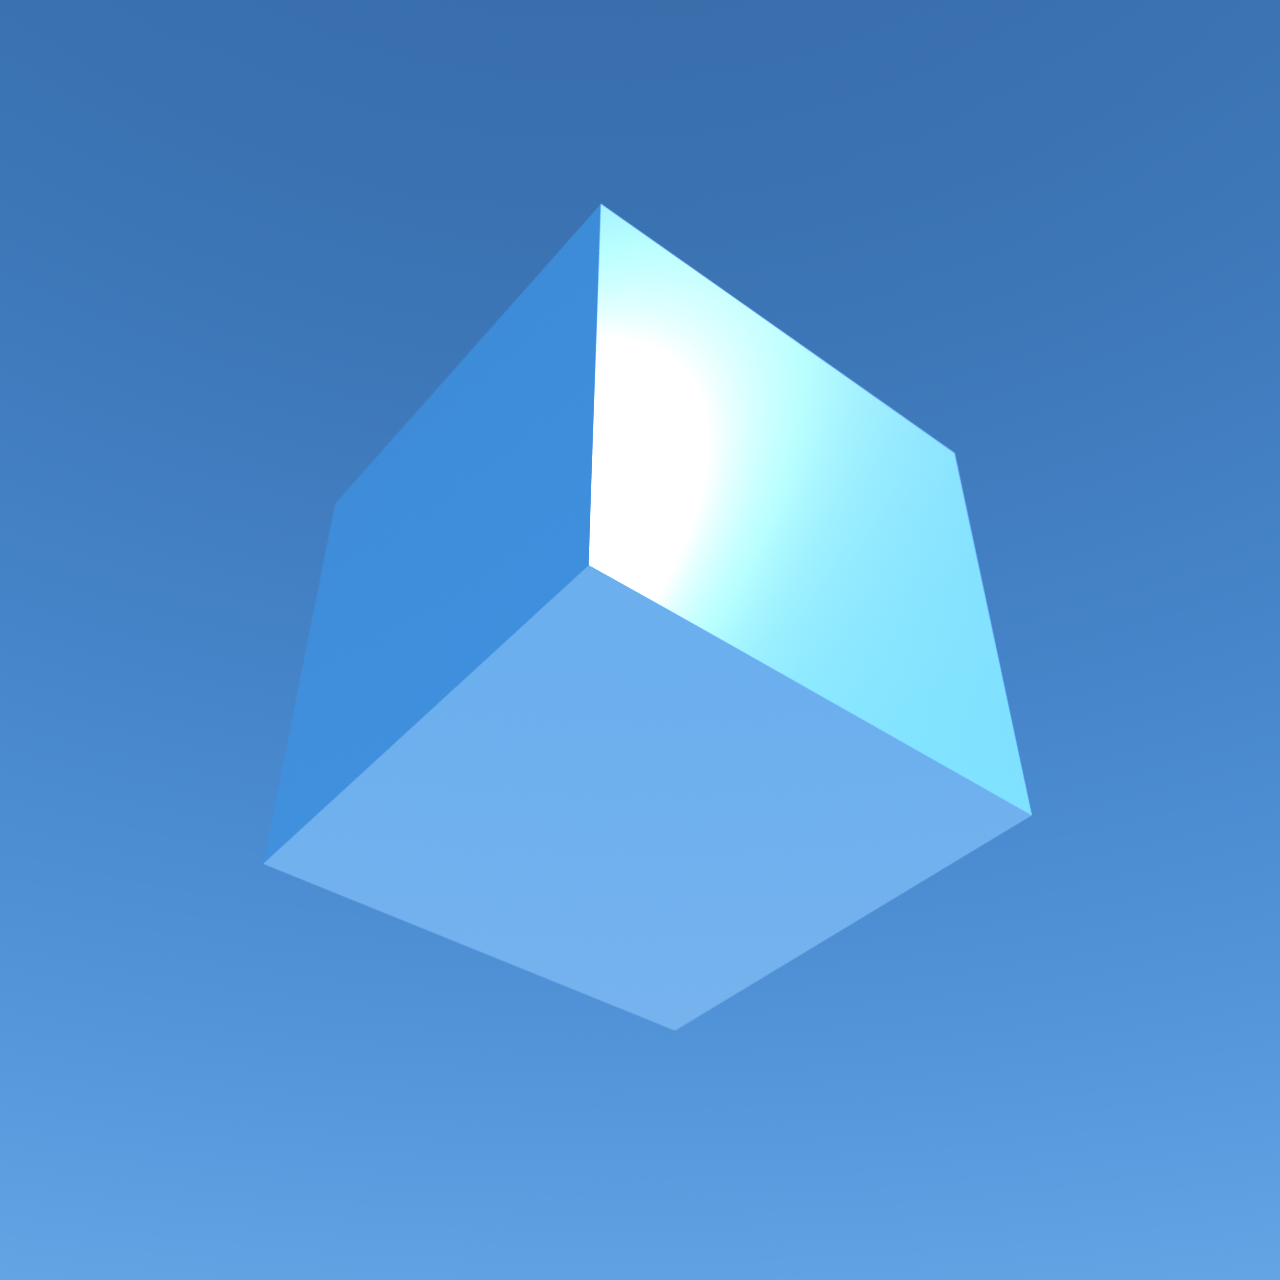
\includegraphics[width=\linewidth]{examples/recipes/architecture-flow/octane-preview.png}
  \caption{MCP architecture flow as spatial geometry.}
\end{subfigure}\hfill
\begin{subfigure}{0.32\linewidth}
  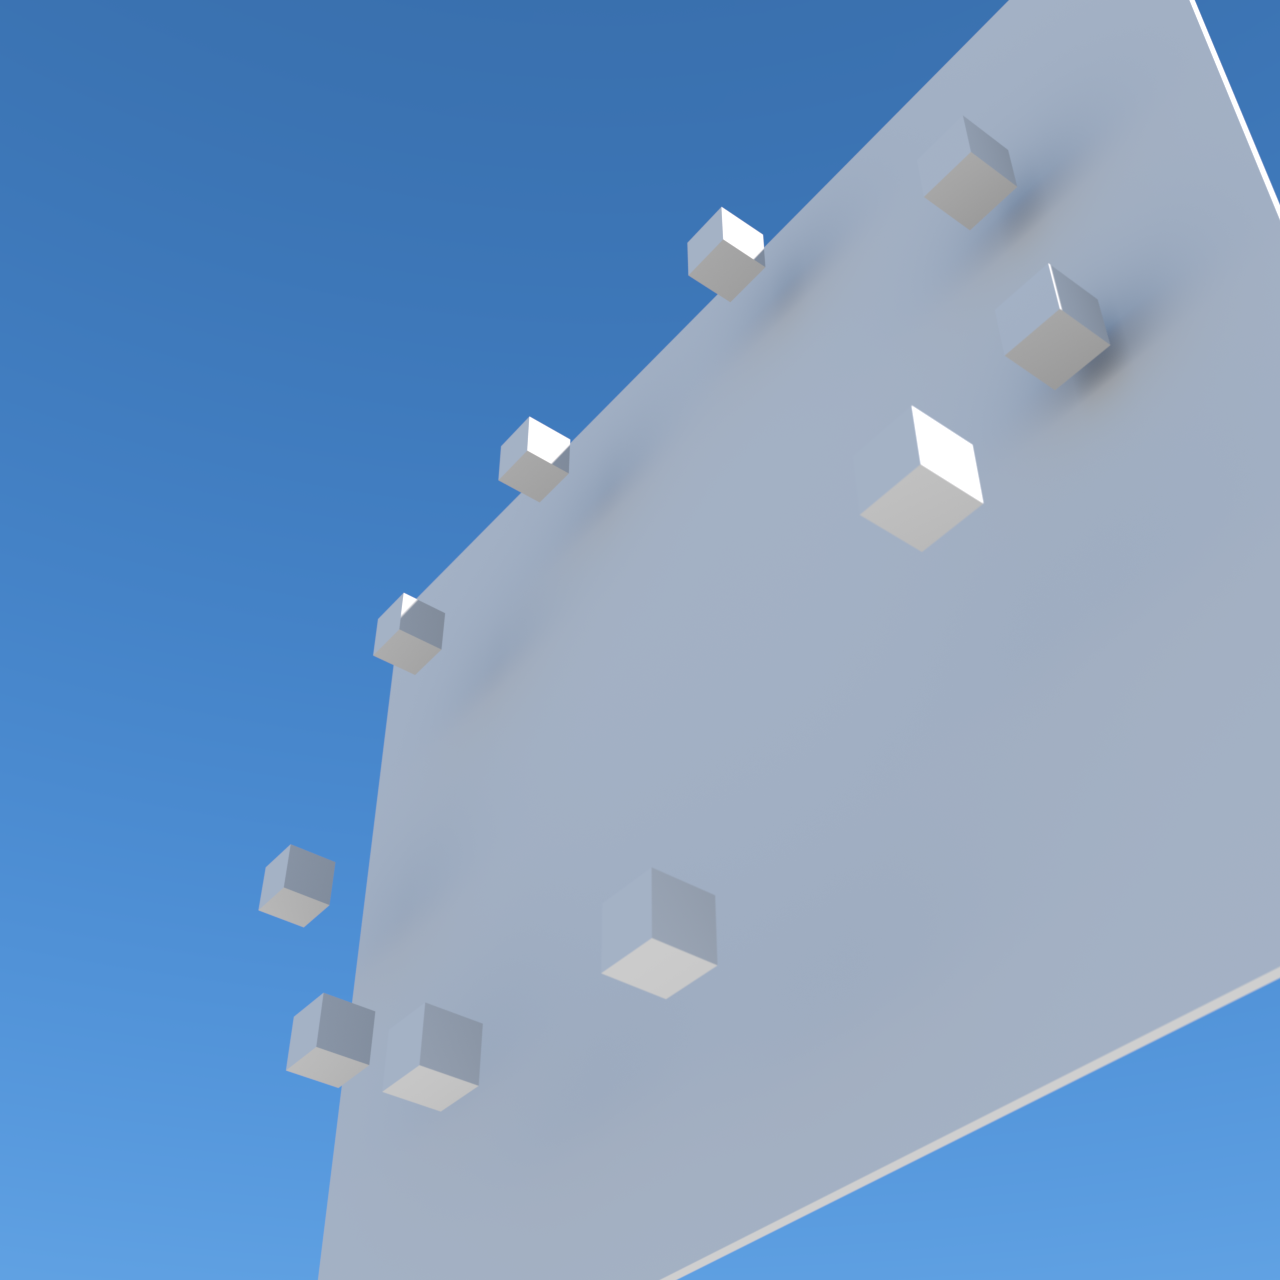
\includegraphics[width=\linewidth]{examples/recipes/network-graph/octane-preview.png}
  \caption{Knowledge graph topology.}
\end{subfigure}
\caption{The corpus includes explanatory diagrams as 3D scenes. This is central to the goal of using Octane X as a communication surface, not merely a photoreal renderer.}
\label{fig:diagram-recipes}
\end{figure}

\subsection{Math and physics recipes}

\begin{figure}[htbp]
\centering
\begin{subfigure}{0.32\linewidth}
  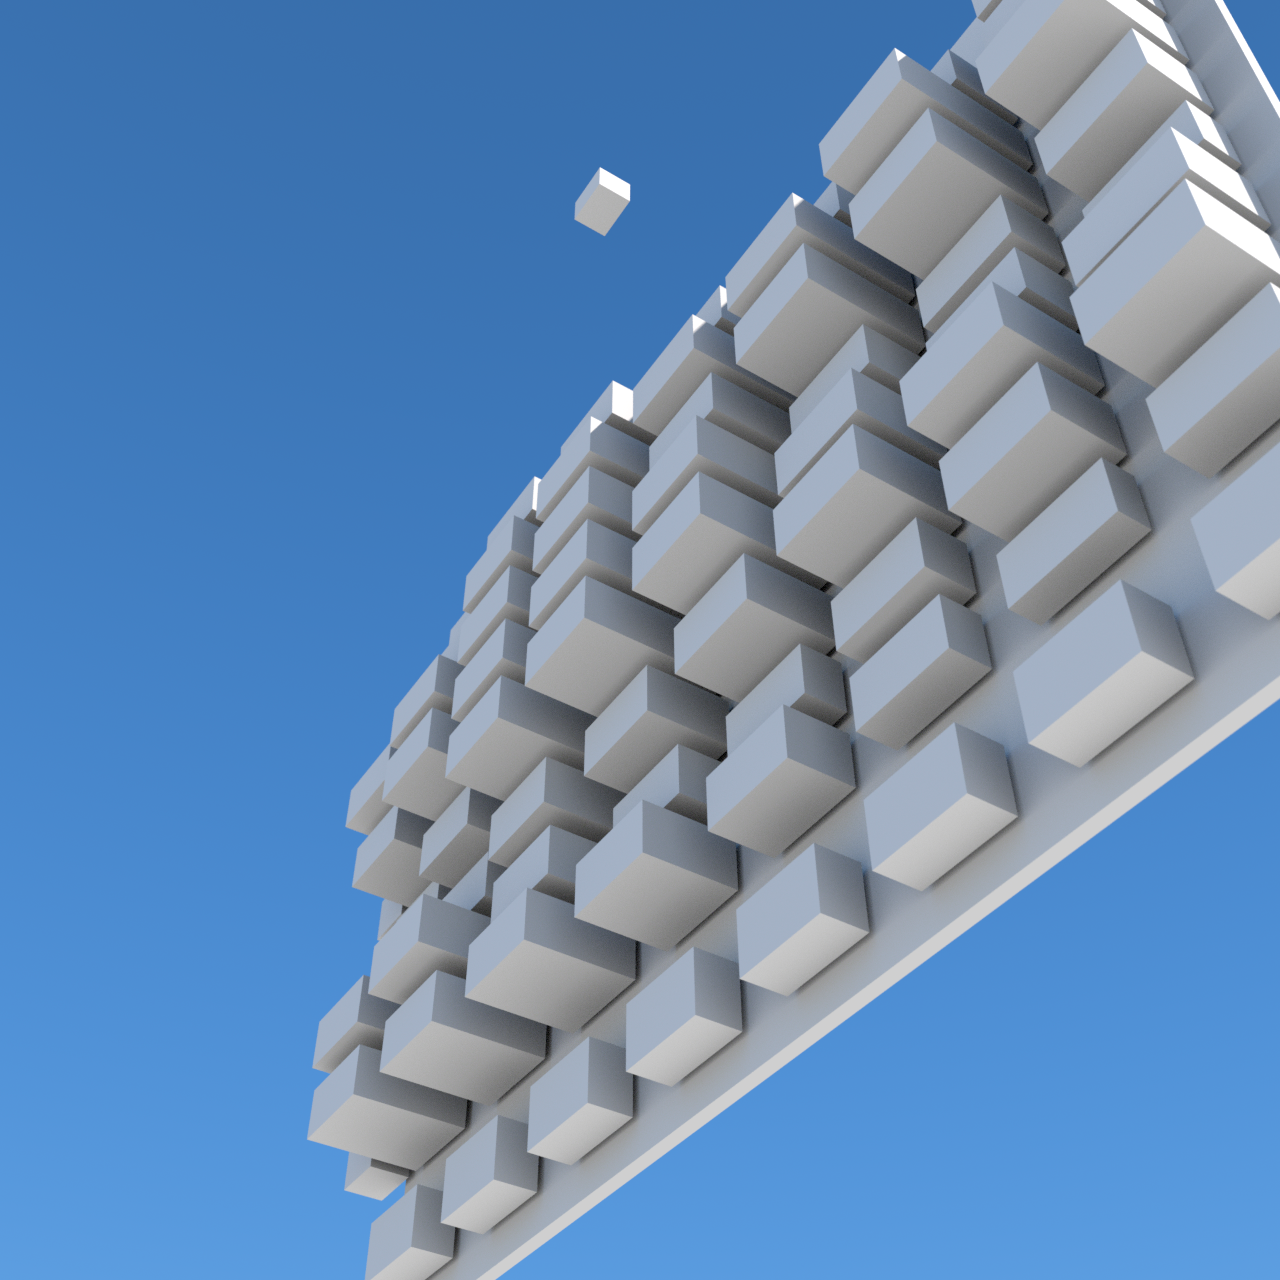
\includegraphics[width=\linewidth]{examples/recipes/vector-field/octane-preview.png}
  \caption{Rotating vector field.}
\end{subfigure}\hfill
\begin{subfigure}{0.32\linewidth}
  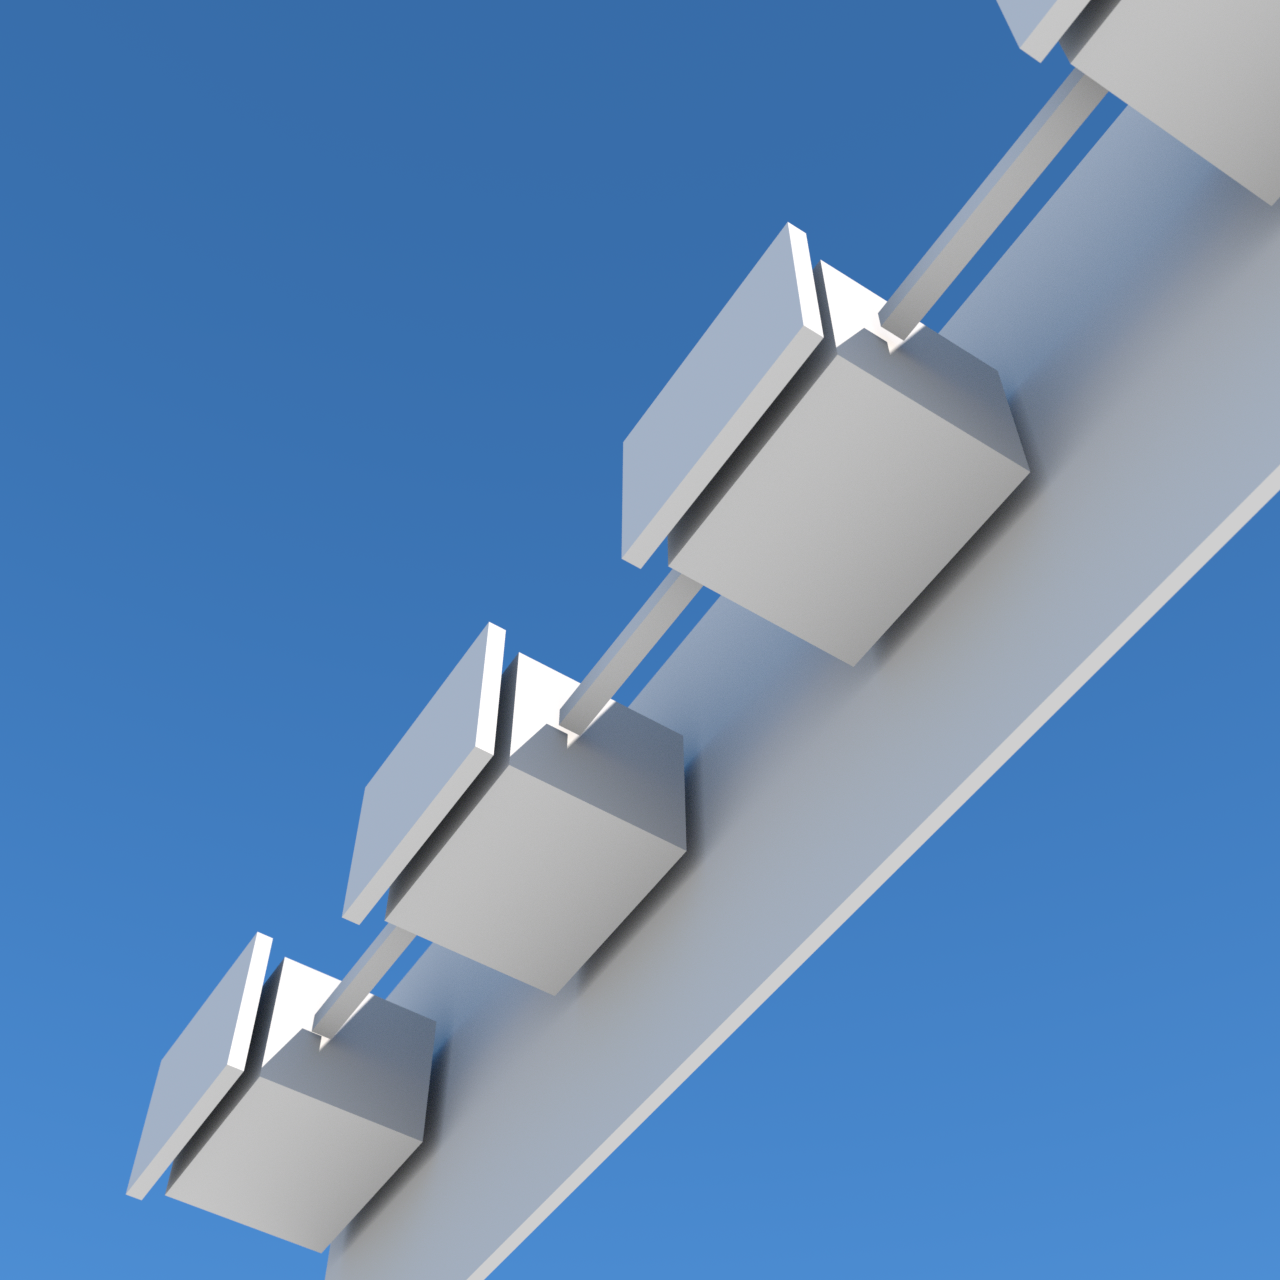
\includegraphics[width=\linewidth]{examples/recipes/wave-interference-field/octane-preview.png}
  \caption{Two-source wave interference field.}
\end{subfigure}\hfill
\begin{subfigure}{0.32\linewidth}
  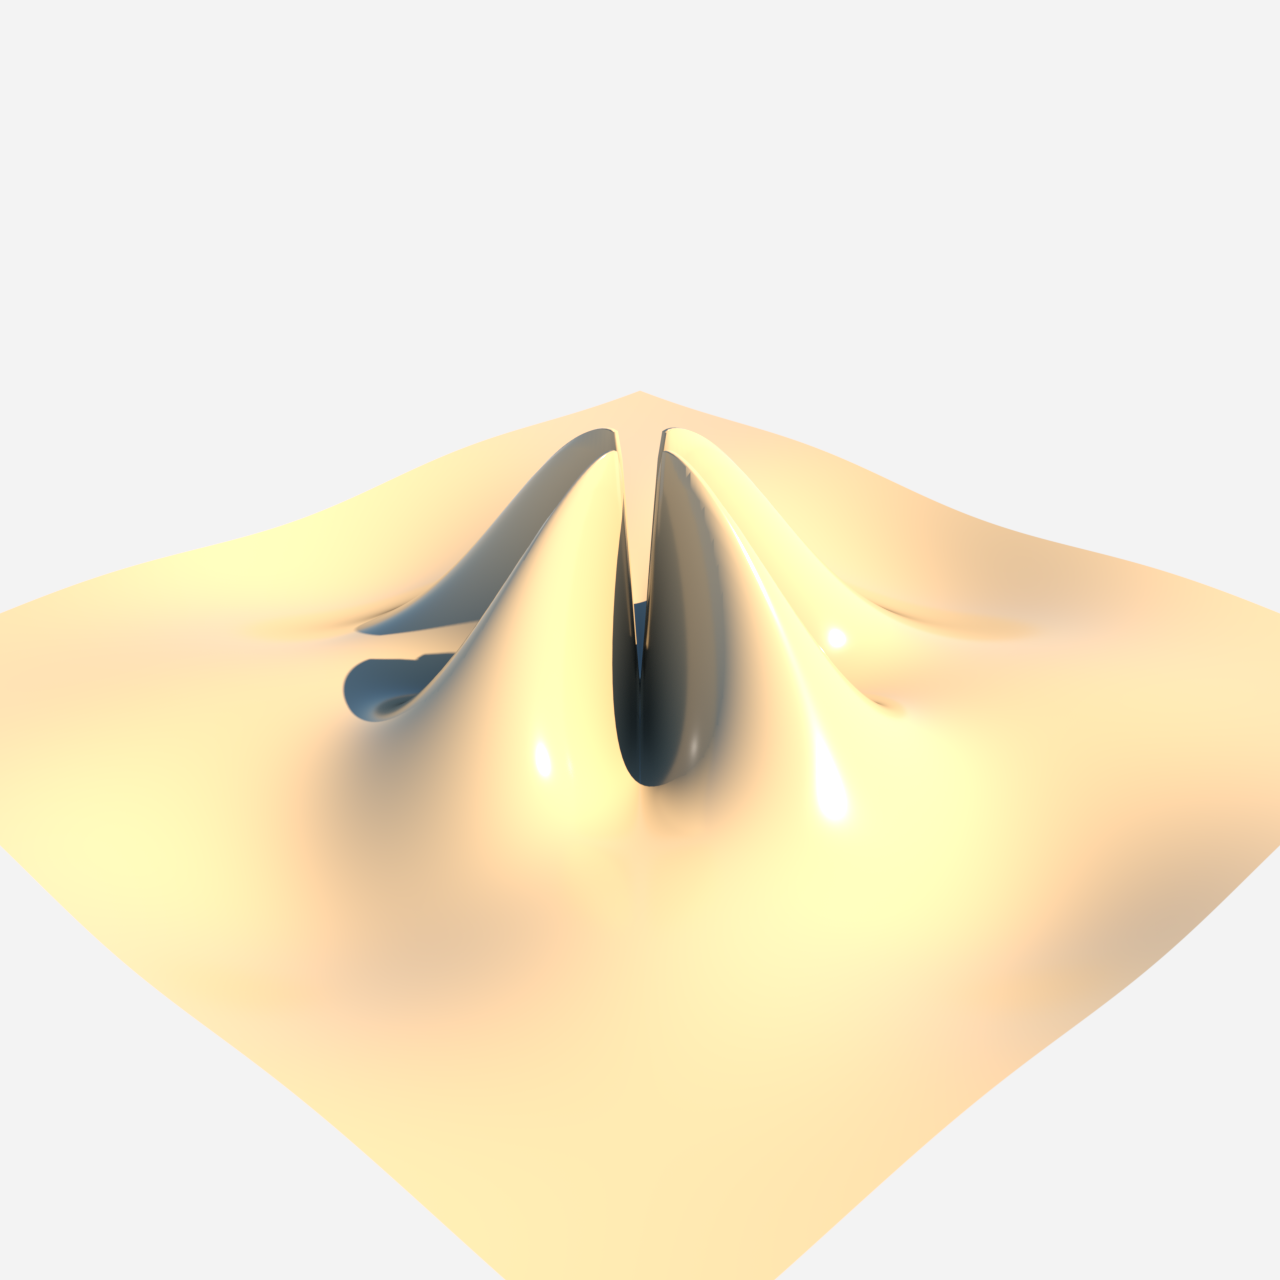
\includegraphics[width=\linewidth]{examples/recipes/math-surface/octane-preview.png}
  \caption{Radial mathematical surface.}
\end{subfigure}
\caption{Mathematical scenes benefit from deterministic mesh generation and bounds-aware cameras. The 3DXM work extends this direction toward a larger library of named mathematical surfaces.}
\label{fig:math-recipes}
\end{figure}

\section{Comparison with other image and model generation toolsets}

\project{} should not be evaluated as a replacement for every image-generation system. It occupies a different design point: explicit, local, renderer-backed, agent-editable scene construction. Table~\ref{tab:comparison} summarizes the trade space.

\begin{longtable}{p{0.18\linewidth}p{0.20\linewidth}p{0.25\linewidth}p{0.25\linewidth}}
\caption{Comparison with adjacent image/model generation toolsets.}\label{tab:comparison}\\
\toprule
\textbf{Toolset class} & \textbf{Strengths} & \textbf{Weaknesses for this use case} & \textbf{Relationship to \project{}} \\
\midrule
\endfirsthead
\toprule
\textbf{Toolset class} & \textbf{Strengths} & \textbf{Weaknesses for this use case} & \textbf{Relationship to \project{}} \\
\midrule
\endhead
Text-to-image models (Stable Diffusion, FLUX, Midjourney-like services) & Rapid aesthetic ideation, style transfer, concept art, broad learned priors. & Geometry is implicit; edits are probabilistic; physical structure, scale, labels, and provenance are hard to guarantee. & Useful for reference images and mood targets, but not the canonical render path for render-intent prompts. \\
\addlinespace
ComfyUI / node graph diffusion workflows & Reusable generation graphs, conditioning, ControlNet/IP-Adapter-style steering, local execution possible. & Still primarily latent-image generation; graph complexity can obscure scene semantics; exact 3D object topology is not guaranteed. & Complementary for texture/reference generation and style exploration. \\
\addlinespace
Blender / bpy / Blender MCP & Open 3D scene graph, scripting, headless rendering, geometry nodes, Eevee/Cycles. & GPL licensing and heavier runtime; distinct API and material system; integration must be isolated carefully. & Strong candidate for an open renderer backend or separate MCP bridge behind the same scene DSL. \\
\addlinespace
WebGL / three.js / React Three Fiber & Realtime, interactive, browser-shareable, MIT-licensed, ideal for Agentic Canvas. & Less photoreal than Octane; requires a web scene representation and snapshot path. & Highest-leverage future preview/shareable backend; can host live data/math scenes. \\
\addlinespace
Godot 4 & Realtime engine, interaction, physics, animation, MIT license. & Game-engine paradigm differs from the OBJ/command queue; less direct for photoreal stills. & Useful for staged interactive concepts if a specific need emerges. \\
\addlinespace
Scientific Python visualization (Open3D, PyVista/VTK, VisPy, trimesh) & Python-native geometry, point clouds, meshes, offscreen renders, data/science workflows. & Usually less photoreal and less polished as final communication art. & Best treated as generator-layer support feeding Octane/WebGL/Blender backends. \\
\addlinespace
Geospatial web engines (CesiumJS, deck.gl, MapLibre) & Native geo primitives, globes, maps, layers, timeseries, browser interaction. & Domain-specific; not a universal render backend. & Natural backend for the geospatial grammar instead of forcing all maps into OBJ. \\
\addlinespace
Open path tracers (Mitsuba, OSPRay) & Scriptable, reproducible quality rendering, research-friendly. & Offline quality tier; setup and material translation work required. & Potential quality-tier alternative where Octane is unavailable or undesirable. \\
\bottomrule
\end{longtable}

The comparison suggests a layered future rather than a single winner. Octane X remains the photoreal quality tier. WebGL/three.js is the likely realtime/shareable tier. Scientific Python and geospatial engines are best viewed as domain generators or specialized backends. Blender and Mitsuba are optional quality alternatives if licensing and integration boundaries are handled carefully.

\section{Design trade-offs and constraints}

\subsection{Why Octane X?}

Octane X provides high-quality GPU path-traced output, strong material rendering, and a professional photoreal target for product, planetary, and scientific scenes. The recipe corpus shows that once the bridge path is working, Octane can produce compelling native previews from generated geometry.

\subsection{Why not only Octane X?}

The same properties that make Octane powerful also make it operationally awkward for agents. The current macOS application does not provide the ideal headless CLI/plugin path for this workflow. The bridge must use a sandbox-aware workspace and Script-menu Lua execution. AppleScript launch requires correct macOS Accessibility permission on the runtime process. Per-frame animation drains can be slow. These are manageable constraints, but they motivate the renderer-abstraction roadmap.

\subsection{Why explicit geometry instead of prompt-only rendering?}

Explicit geometry makes the system debuggable. If a render fails, the agent can inspect face indices, material groups, bounds, camera target, queue contents, command results, preview mtime, and pixel statistics. In prompt-only generation, the same failure is often expressed as another prompt tweak with uncertain causal effect.

\section{Planned developments}

The project roadmap can be grouped into four development tracks.

\subsection{Track A: Bridge hardening}

The immediate technical priority is making bridge behavior less fragile and easier to reason about:

\begin{itemize}[leftmargin=*]
  \item \textbf{Single-source Lua handler generation.} Today the one-shot and persistent bridge entrypoints still inline handler copies. The roadmap calls for a single handler/runtime source or generated chunks with source hashes.
  \item \textbf{Capability-backed material/light registry.} Material and light support should be reported from an Octane API/capability corpus rather than scattered empirical fallback lists.
  \item \textbf{Schema/dispatch parity.} Python allowed operations, payload validators, schema output, and Lua dispatch branches should continue to be guarded by tests.
  \item \textbf{Server-boot verification.} Offline tests are necessary but not sufficient; the real console-script server must boot with the correct environment and expose the expected tool surface.
\end{itemize}

\subsection{Track B: Scene grammar expansion}

The scene manifest should become the main agent-readable representation. Useful next grammar additions include cones, tubes, arrows, polyline tubes, point clouds, text-label placeholders, better transform handling, stable manifest-relative asset paths, and patch operations for iterative edits.

\subsection{Track C: Visual-review loops}

The render-review loop should evolve from a preview checker into an orchestration tool: queue scene, drain/render, review pixels, suggest bounded camera/material/lighting fixes, compare before/after previews, and persist evidence next to the recipe. The principle remains: do not claim a render succeeded unless a real preview file exists and passes the appropriate checks.

\subsection{Track D: Backend abstraction}

The strategic direction is to decouple the scene DSL from Octane X. The proposed backend interface would preserve the current Octane path while adding optional adapters:

\begin{itemize}[leftmargin=*]
  \item \textbf{OctaneBackend}: existing photoreal quality path;
  \item \textbf{WebGLBackend}: live three.js scenes in Agentic Canvas, with snapshot-to-PNG for review;
  \item \textbf{GeoBackend}: CesiumJS/deck.gl style native geo visualization;
  \item \textbf{BlenderBackend}: process-isolated open 3D backend using bpy or Blender MCP;
  \item \textbf{QualityBackend}: Mitsuba/OSPRay-style reproducible path tracing.
\end{itemize}

\section{Future application opportunities}

\subsection{Scientific and geospatial visualisation}

\project{} is well suited to scenes where data must remain inspectable: Earth interior models, gravity/geoid fields, terrain, GeoJSON layers, point clouds, orbital mechanics, vector fields, and mathematical surfaces. The Earth cutaway and geospatial-terrain recipes are early examples; the 3DXM surface work points toward a larger geometry grammar.

\subsection{Research hypothesis communication}

For exploratory hypotheses, the system can render falsifiable visual models rather than rhetorical diagrams. A geophysical claim, for example, can be converted into layered geometry, predicted alignments, control views, and null-model comparisons. This is not proof by rendering; it is a way to make assumptions visible.

\subsection{Agentic product and industrial design}

The product-studio recipes demonstrate object-level iteration. Future work could add parametric object generators, material presets, fabric/metal/glass libraries, and user-steered render variants where feedback is mapped to geometry or material edits.

\subsection{Education and explanation}

Architecture-flow, data-bars, vector-field, and wave-interference recipes show how system architecture, data comparisons, and physical principles can become spatial scenes. A live WebGL backend would make these outputs interactive and shareable.

\subsection{Model evaluation and visual QA}

The benchmark suite demonstrates a path for evaluating render-capable agents. Tasks can isolate failure classes such as blank frames, wrong material group, incorrect geometry topology, clipping, or scene-ordering errors. This could become a broader benchmark for agentic visualization systems.

\subsection{Multi-agent visual studios}

Because the scene state is file-backed, multiple agents can specialize: one generates geometry, one critiques pixel output, one updates documentation, and one manages queue/render scheduling. The repo already contains coordination rules for shared renderer access; future work can formalize this into a multi-agent studio workflow.

\section{Risks and mitigations}

\begin{table}[htbp]
\centering
\caption{Primary risks and current mitigations.}
\begin{tabular}{p{0.28\linewidth}p{0.33\linewidth}p{0.27\linewidth}}
\toprule
\textbf{Risk} & \textbf{Consequence} & \textbf{Mitigation} \\
\midrule
MacOS Script-menu / TCC fragility & Bridge launch fails or appears unavailable. & Document exact Accessibility target; provide doctor/status tools and fallback manual bridge execution. \\
Queue contamination & Stale commands produce misleading renders. & Flush queue before live renders; use lifecycle dirs and mtime/pixel guards. \\
Renderer-specific coupling & DSL becomes too Octane-shaped. & Introduce backend interface while preserving OctaneBackend as first implementation. \\
Vision hallucination & Incorrect render accepted as success. & Use decoded-pixel checks as gate; vision only for human-facing interpretation. \\
Recipe/doc drift & Future agents learn stale behavior. & Maintain recipe book, WIP/roadmap snapshots, parity tests, and pre-commit documentation review. \\
Large/heavy dependencies & Local-first package becomes brittle. & Keep core dependency-light; gate science/geo/harvest extras as optional. \\
\bottomrule
\end{tabular}
\end{table}

\section{Definition of success}

A mature version of \project{} would satisfy the following criteria:

\begin{enumerate}[leftmargin=*]
  \item An agent can describe a scene semantically and receive a validated scene manifest before rendering.
  \item The renderer backend is selectable: Octane for photoreal output, WebGL for realtime interaction, geospatial backend for maps/globes, and optional open renderers for quality alternatives.
  \item Every renderable scene has reproducible assets, command metadata, preview files, and review evidence.
  \item Pixel/structure review catches blank, clipped, stale, and misframed outputs automatically.
  \item Successful scenes become recipes or promoted tools; failed scenes become documented pitfalls and tests.
  \item Smaller/local models can use the docs and recipes without re-discovering bridge quirks.
\end{enumerate}

\section{Conclusion}

\project{} turns rendering from a one-off aesthetic act into an agentic engineering loop. Its key contribution is not merely that Hermes can produce Octane images. The stronger idea is that a local agent can build, inspect, verify, revise, and remember visual artifacts using explicit scene state. That makes the system useful for scientific visualization, research communication, diagramming, product iteration, and future multi-backend visual canvases.

The next phase should focus on bridge hardening, richer scene grammar, backend abstraction, and application-specific generators. Octane X remains the photoreal anchor, but the long-term value is the renderer-independent visual language that the project is beginning to expose.

\appendix
\section{Selected recipe paths}

\begin{itemize}[leftmargin=*]
  \item \texttt{examples/recipes/earth-hemisphere/}
  \item \texttt{examples/recipes/desk-fan/}
  \item \texttt{examples/recipes/headphones-studio/}
  \item \texttt{examples/recipes/photoreal-vase-studio/}
  \item \texttt{examples/recipes/data-bars/}
  \item \texttt{examples/recipes/architecture-flow/}
  \item \texttt{examples/recipes/network-graph/}
  \item \texttt{examples/recipes/vector-field/}
  \item \texttt{examples/recipes/wave-interference-field/}
  \item \texttt{examples/recipes/math-surface/}
  \item \texttt{examples/recipes/photoreal-earth-space/}
  \item \texttt{examples/recipes/saturn-moons-space/}
\end{itemize}

\section{Primary project documents consulted}

\begin{itemize}[leftmargin=*]
  \item \texttt{README.md}
  \item \texttt{docs/roadmap.md}
  \item \texttt{docs/WIP.md}
  \item \texttt{docs/recipe-book.md}
  \item \texttt{docs/recipe-library.md}
  \item \texttt{docs/benchmark-suite.md}
  \item \texttt{docs/agent-quickstart.md}
  \item \texttt{docs/visualization-backends-research.md}
  \item \texttt{examples/recipes/*/scene.json}
\end{itemize}

\end{document}
